\scanpage{76}
% archive foliation: 75
Si on s'intéresse à $E_X$ au lieu de $\underline{\mathcal O}_X$,
il faut remplacer $\underline\omega_X$ par $\underline\omega_X^*$
(\unsure{donc} faisceau des bases de $\underline\omega_X$, i.e. des
\unsure{sections|sects} sans zéros), qui est un torseur
\uline{sous $\underline{\mathcal O}_X^*$}, et $dg-df$ par
\deleted{$\unsure{dg}$} :
\[
A'(f,g)=\frac{dg}{df}\in\Gamma(X,\underline{\mathcal O}_X^*)
\]

b) $G_m$ \uline{agissant sur $\underline E^1$, ou
$\underline E^{1*}\simeq G_m$} par \deleted{translations}
\inserted{homothéties}. Plus \unsure{généralement|général.}, considérons
son opération sur un faisceau inversible $L$, soit $L^*$ le sous faisceau
des bases \inserted{(torseur sous $\underline{\mathcal O}_X^*$)},
on s'intéresse à $L^*/\mathbf C^*$. Or à tt section de $L^*$ est associée
une connexion sur $L$ : on trouve ainsi un hom
\[
L^*\deleted{\unsure{f}}\xrightarrow{D}
\underline{\operatorname{Conn}}_{X/\mathbf C}(L^*)
\qquad(f\longmapsto D_f)
\]
où le dernier est un torseur sous
$\unsure{\underline\Omega^1_{X/\mathbf C}|\underline\omega_{X/\mathbf C}}$,
et ceci induit un \deleted{biject} iso
\[
L^*/\mathbf C^*\simeq\underline{\operatorname{Conn}}_{X/\mathbf C}(L).
\]

Si on ignorait la notion de connexion, on introduirait directement
$B(f,g)$ $(f,g\in\Gamma L^*)$, qui se \unsure{conf.|confond} $D_g-D_f$, par
\[
B(f,g)=\frac{d\,g/f}{g/f}\in\Gamma\underline\omega_{X/\mathbf C}
\]
avec des propriétés du type a) b) c) d) e). Dans le cas
$L=\underline{\mathcal O}_X$,
$\underline{\operatorname{Conn}}(L)\simeq\underline\omega_{X/\mathbf C}$
can., et il suffit de considérer
\[
g\longmapsto\frac{dg}{g}\qquad
\mathcal O_X^*\longrightarrow\underline\omega_{X/\mathbf C}
\]
qui induit
\[
\frac{\underline{\mathcal O}_X^{\unsure{\prime|*}}}{\mathbf C^*}
\simeq\underline\omega_{X/\mathbf C}.
\]
\figure{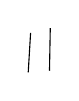
\begin{tikzpicture}[x=1cm,y=1cm]
\draw (0,0)--(0.03,0.50);
\draw (0.27,0.02)--(0.28,0.56);
\end{tikzpicture}}

